% move conc to end section3
\documentclass[sigconf,screen]{acmart}
\usepackage{color, colortbl}
\usepackage{graphicx} % Required for inserting images
\usepackage{dblfloatfix} 
\usepackage{wrapfig} 
\usepackage{balance} 
\usepackage[utf8]{inputenc}
\usepackage{microtype}
\usepackage[normalem]{ulem}
\usepackage[T1]{fontenc}  
 
% \setcopyright{ACMUNKNOWN} 
% \acmPrice{15.00}
% \acmDOI{10.1145/3617555.3617876}
% \acmYear{2023}
% \copyrightyear{2023}
% \acmSubmissionID{fsews23promisemain-p14-p}
% \acmISBN{979-8-4007-0375-1/23/12}
% \acmConference[PROMISE '23]{Proceedings of the 19th International Conference on Predictive Models and Data Analytics in Software Engineering}{December 8, 2023}{San Francisco, CA, USA}
% \acmBooktitle{Proceedings of the 19th International Conference on Predictive Models and Data Analytics in Software Engineering (PROMISE '23), December 8, 2023, San Francisco, CA, USA}

\setcopyright{acmlicensed}
\acmPrice{15.00}
\acmDOI{10.1145/3617555.3617876}
\acmYear{2024}
\copyrightyear{2024}
\acmSubmissionID{fsews23promisemain-p14-p}
\acmISBN{979-8-4007-0375-1/23/12}
\acmConference[PROMISE '24]{EMSE journal extensions of   papers from the  19th International Conference on Predictive Models and Data Analytics in Software Engineering}{December 8, 2023}{San Francisco, CA, USA}
\acmBooktitle{EMSE journal extensions of   papers from the  19th International Conference on Predictive Models and Data Analytics in Software Engineering (PROMISE '23), December 8, 2023, San Francisco, CA, USA}
\received{2023-07-07}
\received[accepted]{2023-07-28}

	

%\date{July 7, 2023}
%\copyrightyear{2023}
%\setcopyright{acmcopyright}
%\acmConference{PROMISE'23: The 19th International Conference of Predictive Models and Data Analytics in SE, December 8, 2023, San Francisco, USA}
%\acmISBN{XX-X-xxxx-xxxx-x/23/112}\acmPrice{\$15.00}

 
 
 
 
\begin{abstract}
To make models more understandable and correctable,   I propose that the PROMISE community pivots to the problem of {\em model review}. 
Over the years, there have been many reports that very simple models can perform exceptionally well. Yet, where are the researchers asking ``say, does
that mean that we could make software analytics simpler and more comprehensible?''
 This is an important question, since humans often have difficulty accurately assessing complex models (leading to unreliable and sometimes dangerous results). 
 
 Prior PROMISE results have shown that data mining can effectively summarizing large models/ data sets into simpler and smaller ones.  Therefore, the PROMISE community has the skills and experience needed to redefine, simplify, and improve the relationship between humans and AI.
\end{abstract}
 
\begin{CCSXML}
<ccs2012>
   <concept>
       <concept_id>10011007.10011074.10011099.10011693</concept_id>
       <concept_desc>Software and its engineering~Empirical software validation</concept_desc>
       <concept_significance>500</concept_significance>
       </concept>
   <concept>
       <concept_id>10010147.10010178.10010205</concept_id>
       <concept_desc>Computing methodologies~Search methodologies</concept_desc>
       <concept_significance>500</concept_significance>
       </concept>
   <concept>
       <concept_id>10010147.10010178.10010216.10010217</concept_id>
       <concept_desc>Computing methodologies~Cognitive science</concept_desc>
       <concept_significance>500</concept_significance>
       </concept>
   <concept>
       <concept_id>10010147.10010257</concept_id>
       <concept_desc>Computing methodologies~Machine learning</concept_desc>
       <concept_significance>500</concept_significance>
       </concept>
 </ccs2012>
\end{CCSXML}

\ccsdesc[500]{Software and its engineering~Empirical software validation}
\ccsdesc[500]{Computing methodologies~Search methodologies}
\ccsdesc[500]{Computing methodologies~Cognitive science}
\ccsdesc[500]{Computing methodologies~Machine learning} 

\keywords{Model, review, discrimination, data mining, optimization}
 
% \input{body-of-your-manuscript}
% \balance
% \bibliographystyle{ACM-Reference-Format}
% \bibliography{name-of-your-bib-file}
% \end{document}
% You should generate the CCSXML code with the tool at http://dl.acm.org/ccs.cfm a

\begin{document}
\title{Model Review: A PROMISEing Opportunity}

\author{Tim Menzies}
\orcid{0000-0002-5040-3196}
\email{timm@ieee.org}
\affiliation{%
  \institution{North Carolina State University}  
  \country{USA}
}
\maketitle
%\pagestyle{plain} 
\section{Introduction}
PROMISE will soon enter its third decade. 
 What have we learned from two decades of PROMISE v1.0 that could shape the next decade of PROMISE v2.0?
 
Over the years, there have been many results
where   very simple models performed exceptionally well~\cite{Holte1993VerySC,menzies2008implications,agrawal2019dodge,Xu21,Tawosi23,Kohavi97}.
Using those results,   PROMISE v2.0 could focus less on model creation,  and more on something that requires and demands simpler and more comprehensible models. 
Specifically, I say PROMISE v2.0 should be about simplifying  {\em model review} (using data mining).


% It may seem disingenuous, even dishonest, when someone warns of a problem that they themselves have caused. For example, President Eisenhower's 1961 farewell address warned on the dangers of the military-industrial complex\footnote{Eisenhower said ``We must guard against the acquisition of unwarranted influence, whether sought or unsought, by the military-industrial complex. The potential for the disastrous rise of misplaced power exists and will persist.''}-- an institution that was partially brought about by his administration's budget priorities.  

% I say this since the theme of this paper is that there are problems with the PROMISE conference series; and that I am (partially)
% responsible for those problems.  Mea culpa.
% But the good news is that, in my view, these problems can be fixed using tools developed from the PROMISE experience.




\section{  Why Change   PROMISE?}

  PROMISE v1.0 was created one night in 2004 walking around Chicago's Grant Park. Jelber Sayyad-Shirabad and I had spent the day at a disappointing workshop
on data mining and SE. ``Must do better'', we said.  ``Why don't we do it  like in ML? Make conclusions reproducible? Demand that if people publish a paper, they should also publish the data used in that data?"\footnote{
In 2023 it is  hard to believe that ``reproducible SE'' was a radical idea.  But once upon a time, there was little sharing of data and scripts-- so much so that in 2006 Lionel Briand predicted the failure of PROMISE saying ``no one will give you data''.}.

At first, the series got off to a shaky  start. But once
Elaine Weyuker, Thomas Ostrand, Gary  Boetticher, and Guenther Ruhe
joined the steering committee, the meeting earned the prestige needed for future  growth.
And
in those early days, it
was impressive to see so many researchers
taking up the idea of reproducible results.
Numerous papers were written that applied an increasing
elaborate tool set to data like COC81, JM1, XALAN, DESHARNIS
and all the other data sets that were used (and reused) in the first decade of PROMISE.

Many of those papers lead to successful research. In 2018, 20\% of the articles listed in {\em Google Scholar Software Metrics} for {\em IEEE Transactions
on SE} used data sets from the first decade of PROMISE. So while other research areas struggled to obtain reproducible results, PROMISE swam (as it were) in an ocean of reproducibility.

The problem was that in the second decade of PROMISE, many researchers still continue that kind of first-decade research. For example,   all too often, I must review papers from authors who think it is valid
to publish results based on (e.g.) the COC81 data set first published in 1981~\cite{Boehm1981}; the DESHARNIS data set,  first published in 1989~\cite{desharnais1989analyse}; the JM1 data, first published in 2004~\cite{menzies2004good}; or the XALAN data set, first published in 2010~\cite{jureczko2010towards}\footnote{Just to be clear,
there is value in   a publicly accessible collection of reference problems. For instance, if a PROMISE author is unable to present results from confidential industrial data, they can use the reference collection to construct a reproducible example of their technique. That said, I am usually tempted to reject papers that are {\em solely} based on defect datasets that I contributed to the PROMISE repository in 2005 (e.g. CM1, JM1, KC1, KC2, KC3, KC4, MC1, MC2, MW1, PC1, PC2, PC3, PC4 and PC5)
since, in 2023 we have access to much more recent data
(e.g. see the 1100+ recent Github projects
used by Xia et al.~\cite{xia22}).}.
 

% Another conclusion from the first decade of PROMISE was that we might have been exploring the wrong problem. As noted in an editorial on the best papers from PROMISE 2011~\cite{10.1016/j.infsof.2013.03.006}, the initial belief was that as we collected more data, PROMISE researchers could decrease the variance in their conclusions. However, the opposite turned out to be the case: the {\em more} data we collected,
% the {\em more diverse} that data became and the {\em larger} were the measured variances. I
% tried explaining this, saying   SE learning should focus on  
%  local clusters and not  global models~\cite{menzies2011local,menzies2012local}. Others agreed ~\cite{10.1145/2372251.2372256,bettenburg2012think} while others found no evidence that local models generated better
% predictions than global models~\cite{herbold2017global}.   





% @inproceedings{canfora2013multi,
%   title={Multi-objective cross-project defect prediction},
%   author={Canfora, Gerardo and De Lucia, Andrea and Di Penta, Massimiliano and Oliveto, Rocco and Panichella, Annibale and Panichella, Sebastiano},
%   booktitle={2013 IEEE Sixth International Conference on Software Testing, Verification and Validation},
%   pages={252--261},
%   year={2013},
%   organization={IEEE}
% }
 
Meanwhile, AI fever took over SE. As of 2018,
it became standard at ASE, FSE, ICSME, ICSE, etc. to see papers
that make much use of AI. For example, the MSR conference (which in the early days looked like a sister event to PROMISE) has grown to a large annual A-grade venue.
And just as MSR grew, so did PROMISE shrink. In 2008, PROMISE was a two-day event with 70 attendees. PROMISE is now a much smaller and shorter event. Without definitive results or a novel technological position, it became difficult to differentiate PROMISE from dozens of other, somewhat more prominent, venues.


\section{  Why Switch to  Model Review?}


Reducing the size of the model is an important part of model review.
According to psychological theory~\cite{czerlinski1999good, gigerenzer1999good, martignon2003naive, brighton2006robust, martignon2008categorization, gigerenzer2008heuristics, phillips2017FFTrees, gigerenzer2011heuristic,neth2015heuristics},
humans can best review a system when it ``fits'' it into their memory; i.e., when that it comprises many small model
fragments. 
 Larkin et al.~\cite{Larkin1335} characterize human expertise by a very large long-term memory (LTM)
and a very small short-term memory (STM) that contains as few as four to seven items\footnote{Ma et al.~\cite{ma2014changing} 
 have used evidence from neuroscience and functional MRIs to
argue that the capacity of the STM could be better measured using other factors than ``number of
items ``''. But even they conceded that ``the concept of limited (STM) has considerable
explanatory power for behavioral data''.}.
The LTM contains  many tiny rule fragments
that explore the contents
of the STM to say ``when you see THIS, do THAT''.
When an LTM rule triggers,  can rewrite the STM content, which,
in turn, can trigger other rules.
Experts are experts, says Larkin et al.~\cite{Larkin1335} because LTM patterns dictate what to do, without having to pause for reflection. Novices perform worse than experts,
says Larkin et al., when they fill up their STM with too many to-do's where they plan to pause and reflect on what to do next.  
This theory is widely endorsed.  
 Phillips et al.~\cite{phillips2017FFTrees} discuss how models with tiny fragments can be quickly comprehended by emergency room physicians making rapid decisions; or by guard soldiers making snap decisions about whether to fire or not on a potential enemy; or by stockbrokers making instant decisions about buying or selling stock. 

Complex models cannot fit into STM, leading   to problems with model review.
Green~\cite{green2022flaws}  comments that when faced with large and complex problems,
  cognitive theory~\cite{simon1956rational} tells us that humans use heuristic ``cues'' to lead them to the most important parts
of a model.   Such cues are essential if humans are to reason about large problems.   That said,  using cues can introduce their own errors:
   {\em 
   ...people (including experts) are susceptible to ``automation bias'' (involving) omission errors - failing to take action because the automated system did not provide an alert - and commission error}~\cite{green2022flaws}.
 This means that oversight can lead to the opposite desired effect by {\em ``legitimizing the use of faulty and controversial (models) without addressing (their fundamental issues'')}~\cite{green2022flaws}. 

By ``faulty and controversial models'', Green refers to
the  long list of examples where detrimental models  were learned via
algorithmic means.
For example,   Cruz et al.~\cite{cruz2021promoting}  lists examples where:
\begin{itemize}
\item Proposals from low-income groups are five times more  likely     to be incorrectly ignored by donation groups;
\item Women can be five times more likely to be incorrectly classified as low-income;
\item African Americans are five times more likely to  languish in prison until trial,
rather given the bail they deserve.  
\end{itemize}
These are just a few of the many reported examples\cite{rudin2019explaining}\footnote{See also 
\url{http://tiny.cc/bad23a}, \url{http://tiny.cc/bad23b}, \url{http://tiny.cc/bad23c}} of algorithmic discrimination.
For another example, the last chapter of Noble~\cite{noble2018algorithms} describes how a successful
hair salon went bankrupt due to internal
choices within the YELP recommendation algorithm.

Like
Mathews~\cite{mathews23}, I am not surprised that so many models are unfair. 
Mathews argues that everyone seeks ways to exploit some advantage for themselves. Hence, we should
expect that the software we build to discriminate against some social groupings;
\begin{quote}

{\em 
    ``People often think of their own hard work or a good decision they made. However, it is often more accurate to look at advantages like the ability to borrow money from family and friends when you are in trouble, deep network connections so that you hear about opportunities or have a human look at your application,  the ability to move on from a mistake that might send someone else to jail, help at home to care for children,  etc. The narrative that success comes from hard work misses that many people work hard and never succeed. Success often comes from exploiting a playing field that is far from level and when push comes to shove, we often want those advantages for our children, our family, our friends, our community, our organizations.''}
 \end{quote}
% Mathews understand the root cause of this discrimination, we must first understand that   AI software is still software.
% In a 2015 talk   Sculley et al.~\cite{SculleyHGDPECYC15}  offered Figure~\ref{google} which
% represents the size (in lines of code) of Google’s software suite. Note how small the AI box is, buried away in the middle of all of the other software.  More recently, 
%  Amershi et al. (from   Microsoft~\cite{8804457}) describe their industrial-AI work as a nine-step pipeline.  In that pipeline, only the   model training
%  (which Amershi et al. describe as ``a morning's work, each week'')
%  might be called core AI while the other steps in the pipeline would be familiar to any software engineer who has worked with databases (for example, there first three steps
% are about requirements, data collection, and data cleaning).  
% \begin{figure}[!t]
% \centering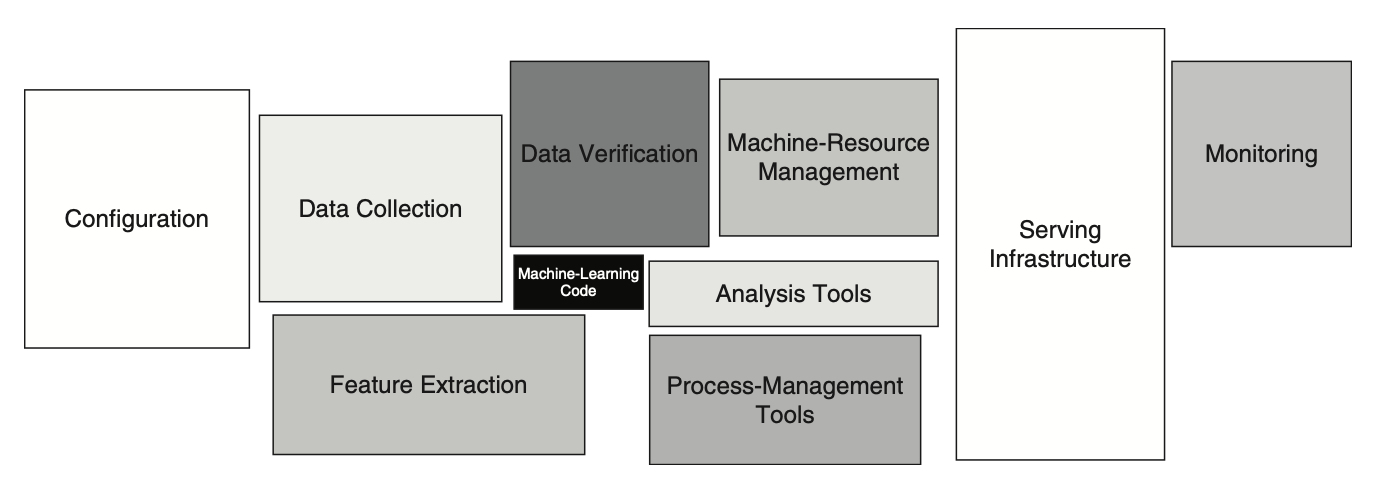
\includegraphics[width=3.5in]{img/x.png}
% \caption{Lines of code, AI-related systems at Google in 2015~\cite{SculleyHGDPECYC15}.
% The tiny black square in the middle is ``core AI'' and the rest are  the standard components of cloud-based S.}\label{google}
% \end{figure}
% Since AI software is software, then the   problems with SE are also problems with AI.
% For example, 
% Conveniently,
% in a ``ship-it'' oriented culture, products are being produced too fast for anyone to
% detect products promoting an unfair advantage.
% With the arrival of generative AI, this trend is  sure to get worse. In the currently AI culture, many products are oriented around large language models that very few people can review, critique or improve. 
Hence I assert that
unfairness is a widespread issue that needs to be addressed and managed. 
Specifically, we need 
to ensure that a software system created by one group, $A$, can be critiqued and modified by another group, $B$.
There are many ways to do this and at PROMISE'23, it is appropriate to focus on the data mining methods issues
(see next section). 

But first, we take care to stress that technical methods like data mining should not be used in isolation.
 PROMISE v2.0 should acknowledge its
   relationship and   responsibilities to those affected by the tools we deliver. We must stop ``flattening'', which is the trivialization and even ignoring of legitimate complaints that our institutions discriminate against certain social groups~\cite{Coaston19}. Bowleg~\cite{doi:10.2105/AJPH.2020.306031} warns that flattening ``depoliticized and stripped (its) attention to power, social justice, and (how we do things wrongly)''.
   
To address these issues, organizations should review their hiring practices to diversify the range of perspectives seen in design teams.  Requirements engineering practices should be improved to include extensive communication with the stakeholders of the software. 
 Software testing teams should extend their tests to cover issues such as discrimination against specific social groups~\cite{cruz2021promoting,10.1145/3585006,Chakraborty}. 
 
Further, on the legal front,
Canellas~\cite{canellas21} and Mathews et al.~\cite{matthewsshould} suggest a tiered process in which the most potentially discriminatory projects are routinely reviewed by an independent external review team
(as done in the IEEE 1012 independent V\&V standard). Ben Green~\cite{green2022flaws} notes that reviewing software systems and AI systems is becoming a legislative necessity and that human-in-the-loop auditing of decisions made by software is often mandatory.
Such legislation is necessary to move away from the internal application of voluntary industrial standards (since, as seen in the Volkswagen emissions scandal (see \url{http://tiny.cc/scandalvw}), companies cannot always be trusted
to voluntarily apply reasonable standards.  

 

\section{How To Make Smaller Models?}

How to make models smaller, more comprehensible, and easier to review?
 Enter all the data mining tools explored at PROMISE.
In those explorations, often it was seen that

 \centerline{\bf A small number of \underline{key} variables control the rest.}
 \noindent
Just to state the obvious, there is a clear
connection between  keys and the  cognitive effort needed  better review methods. Specifically: for a system
with keys, we only need to look
at a few keys to 
  understanding and/or critique and/or control  that system. 

Outside of SE, I have seen keys in hospital nutrition analysis~\cite{partington2015reduced} and avionic control systems~\cite{gay2010automatically}. Within SE, I have seen keys in:
\begin{itemize}
 \item  
Defect prediction datasets~\cite{menzies2006data} where two to three attributes were
enough to predict for defects
\item
Effort estimation models~\cite{chen2005finding} where four to eight attributes
where enough to predict for defects;
\item 
Requirements models for NASA deep space missions~\cite{jalali2008optimizing} where
two-thirds of the decision attributes could be ignored while still finding effective 
optimizations; 
\item
11 Github issue close time data sets~\cite{rees2017better}  
where only 3 attributes (median) were needed for   effective prediction.
\end{itemize}
One way to see how many keys are in a system is to ask how many {\em prototypes} (minimum number of examples)  are required to explore that system. 
At PROMISE"08, the keys were found in 50
examples (selected at random) since the models built from this small sample performed no worse than the models learned from thousands of additional examples~\cite{menzies2008implications}.  
In 2023 we made a similar observation. 
In a study that explored 20 years of data from 250 Github projects with 6000 commits per project (average).
In that study, the defect models learned from only the first 150 commits were predicted, as well as the models learned from much larger samples~\cite{10.1145/3583565}.

\begin{table}[!t]
\caption{Recursive bi-clustering for  model review. Here,
to explore (say)  $N=10,000$ examples, we would only need to pose  \mbox{$2\log_2(N)<30$} questions about
a handful of attributes.}\label{stealth}
\begin{tabular}{|p{.98\linewidth}|}\hline
\rowcolor{blue!10}
My preferred 
recursive bi-clustering procedure is  based on the FASTMAP Nystr{\"o}m algorithm~\cite{faloutsos1995fastmap,platt2005fastmap,papakroni2013data}. \\
This method maps points to the dimension
of greatest variance, computed as follows. Find any point.
Finds its furthest neighbor $A$, then finds $A$'s furthest neighbor
$B$. Map all other   points $X$   to the line  $\overline{AB}$ using 
$x=(a^2+c^2-b^2)/(2c)$ where $a,b,c$=${\mathit dist}(X,A), {\mathit dist}(X,B), {\mathit dist}(A,B)$. 
After mapping, we divide the data on the median $x$ value.
 \\
 \rowcolor{blue!10} The generation of contrast rules can then be used to report the minimal differences that
most distinguish the  {\em desired} and {\em current} leaf clusters. Specifically,
treat two leaf clusters {\em current} and the {\em desired} as a two-class
system. Using data just from those two clusters,
apply supervised discretization based on entropy to convert all attributes
into ranges. For ranges that appear
at frequency $x>0$ in the {\em desired}, rank them according to their frequency
$y$ in the {\em current}   using $x^2/(x+y)$.
  Build rules by exploring
all combinations of the (say) $N=10$ top-ranked ranges. 
\\
Pruning heuristics can be used to report only the essential differences in the data.
In greedy pruning {\em},
the distant points $A,B$ are evaluated, and we only recurse on the data nearest
the best point. In 
{\em non-greedy pruning}, the whole tree is generated (without
evaluations). $A,B$ evaluation and pruning is
then applied to the largest subtrees with the fewest differences within the most
variable attributes. This is repeated to generate survivors $\sqrt{N}$,
which are then explored with the greedy approach~\cite{lustosa2023optimizing}.\\\hline
\end{tabular}

\end{table}
% I recommend this
% approach for model review since it can explore
% a  large multi-objective space using just  a few questions 
% (e.g., for $N=10,000$ examples, ask only \mbox{$2\log_2(N)<30$} questions about
% a handful of attributes). 



Of course, not all data sets can be explored by a few dozen keys. 
Recently,  we have successfully modeled security violations in 28,750 Mozilla functions with 271 exemplars and 6000 Github commits using just 300 exemplars~\cite{yu2019improving}\footnote{Specifically, after   incremental active
learning, the SVM had   under 300 support vectors.}. Although 300 is not an especially small
number, it is small enough so that, given (say) two analysts and a month, it would be possible
to review them all.

\begin{wrapfigure}{r}{1.25in}
  \includegraphics[width=1.25in]{aof.png}
\caption{Fairness vs. accuracy from 10,000   hyperparameter options~\cite{cruz2021promoting}. ``A'' is desirable but ``B'' is probable.}\label{one}\end{wrapfigure} Note that keys  have obvious implications for software testing. Ling~\cite{ling2023benefits} generates test suites for cyberphysical systems by first finding prototypes. In that work, $N$  candidate  tests are recursively bi-clustered
  to leaves of size $\sqrt{N}$ (using the methods of Table~\ref{stealth}).
Test suites generated from the mode of each cluster are  orders of magnitude faster to generate and just as effective as tests generated
by   more complex (and slower)
methods.


This recursive bi-clustering method has
also been applied to multi-objective
optimization~\cite{agrawal2020better}.   Given
a large enough initial population (e.g. $N=10,000$), recursive bi-clustering is faster and finds better solutions than state-of-the-art genetic algorithms and sequential
model optimization methods~\cite{Chen19,lustosa2023optimizing}
(even though it only evaluates $2\log{10,000}=26$ examples while other methods
might evaluate 100s to 1000s of examples). 



Once we have a keys-based multi-objective optimizer, we can offer much support for reviewing models with respect to their fairness.
Figure~\ref{one} comes from Cruz et al.~\cite{cruz2021promoting}.
  That figure 
 shows the effects of 10,000 different   hyperparameter   options applied to five
machine learning algorithms
(random forest; LinReg;
boosted trees; decision trees; feed-forward NN)\footnote{The hyperparameters of     Random Forests,       learners
include
(a)~how many $T$   trees to build (e.g., $T\in \{10,20,40,80,160\}$); (b)~how many features $F$
to use in each tree (e.g., $F \in{2,4,10,20,
\mathit{sqrt}, \mathit{log2}, \mathit{all}}$);
(c)~how to  poll the whole forest (e.g., {\em majority} or {\em weighted majority}); 
(d)~what impurity measures (e.g., {\em gini} or {\em entropy} or {\em log.loss}); (e)~what is the minimum examples needed to branch a sub-tree
(e.g., {\em min}$\in \{2,5,10,20,50,100\}$; (f)~should branches be {\em binary} or {\em n-arty}.
In all, this gives us
$5*7*2*3*6*2 > 2,500$ different ways, just to configure a learner in Figure~\ref{one}. }. 
Adjusting tunings  can change 
learners from   low to   high accuracies and fairness (measured here as the ratio of false
positives between different social groups, such as men and women).   
But with the search methods of the Table~\ref{stealth},
reviewing all those points would require just 20 evaluations-- a number so small that (potentially) it could happen between coffee breaks of a stakeholder review session. 








\section{What to Publish at PROMISE v2.0?}

Having presented the methods of the last section,
I rush to add that they are hardly complete.  There is much here that could be better defined/ refined/ improved/ replaced by further research in PROMISE v2.0.

In my view, the goal of a PROMISE v2.0 paper could be ``less is more''; that is, achieve faster, simpler,
better results using some simplification of the existing technique. There are many ways this could be done; e.g. with:
\begin{itemize}
\item Semi-supervised learning methods that let us do much more with much less data~\cite{tu2021frugal,zhu2005semi};
\item Instance or feature selection  to reduce   training data~\cite{olvera2010review,Kohavi97};
\item Distillation methods   reduce model size. For example, a new data set could be synthesized from the branches of a decision tree. By summarizing this new data set, do we find a smaller model? And for alternative neural approaches, 
see~\cite{Shi23,Biswas23}.
\item  {\em Variance studies}
that tests if the improvement of a complex method over a simpler one are   statistically insignificant;
\item Ablation studies~\cite{yedida2023find} to see how
much can be thrown away (of the modeling method, of parts of the training data) while preserving model performance.
\item Studies showing that (say) a 10\% implementation can perform nearly as well as 100\% of an entire system.
\item Some kind of keys-based approach (e.g. see last section).
\end{itemize} 
Human-in-the-loop studies would also be strongly encouraged
in PROMISE v2.0, to test if the smaller models are still acceptable and useful for people. But in line with PROMISE's long
and admirable history of reproducibility, these experiments should
include human surrogates (developed perhaps via data mining)
that can model the strengths and weaknesses of subject matter
experts (and surrogates should be shared as part of the reproducibility package of a paper).

Also encouraged would be a broader range of performance criteria than just (e.g.) accuracy,
Performance should be measured in a multidimensional
manner and include much more than mere predictive performance,
but also runtime, energy usage, discrimination measures, model development cost, etc.


% Just to give a sense of what might appear at PROMISE v2.0, consider my favorite recursive bi-clustering procedure based on the FASTMAP Nystr{\"o}m algorithm~\cite{faloutsos1995fastmap,platt2005fastmap,papakroni2013data}. This method maps points to the dimension
% of greatest variance\footnote{Computed as follows. Find any point.
% Finds its furthest neighbor $A$, then finds $A$'s furthest neighbor
% $B$. Map all other   points $X$   to the line  $\overline{AB}$ using 
% $x=(a^2+c^2-b^2)/(2c)$ where $a,b,c$=${\mathit dist}(X,A), {\mathit dist}(X,B), {\mathit dist}(A,B)$.}
% then divides the data at the median value. The generation of contrast rules can then be used to report the minimal set  differences that
% most distinguish {\em desired} and {\em current} leaf clusters\footnote{Treat  two leaf clusters {\em current} and the {\em desired } as a two-class
% system. Using data just from those two clusters,
% apply supervised discretization based on entropy to convert all attributes
% into ranges. For ranges that appear
% at frequency $x>0$ in the {\em desired}, rank them according to their frequency
% $y$ in the {\em current}   using $x^2/(x+y)$.
%   Build rules by exploring
% all combinations of the (say) $N=10$ top-ranked ranges. }. Pruning heuristics\footnote{In  {\em greedy pruning},
% the distant points $A,B$ are evaluated and we only recurse on the data nearest
% the best point. In 
% {\em non-greedy pruning}, the whole tree is generated (with no
% evaluations). $A,B$ evaluation and pruning is
% then applied to the largest subtrees with the fewest differences within the most
% variable attributes. This is repeated to generate survivors $\sqrt{N}$,
% which are then explored with the greedy approach~\cite{lustosa2023optimizing}.}
% can be used to only report the essential differences in the data. I recommend this
% approach for model review since it can explore
% a  large multi-objective space using just  a few questions 
% (e.g., for $N=10,000$ examples, ask only \mbox{$2\log_2(N)<30$} questions about
% a handful of attributes). 


% Of course, there are many alternatives to the technology in the last paragraph, and PROMISE v2.0 could usefully spend its time critiquing/ faulting/ improving/ replacing
% that approach. B


 


% Artificial Intelligence has revolutionized numerous industries, yet several open problems persist. These challenges include transparency and interpretability of AI models, robustness to adversarial attacks, ethical concerns, data biases, and the ability to handle edge cases effectively. We argue that by leveraging conventional software analytics techniques, we can make significant strides in resolving these open problems.
% AI models, especially deep neural networks, often operate as "black boxes," making it challenging to understand their decision-making processes.

% This lack of transparency and interpretability raises concerns, especially in critical domains such as healthcare and finance, where accountability and trust are paramount. Additionally, the robustness of AI models against adversarial attacks remains a major concern, as even small perturbations in input data can lead to significant misclassifications. Ethical considerations, fairness, and biases in AI systems further compound these challenges. Lastly, the ability to handle edge cases effectively is crucial for deploying AI systems in real-world scenarios.









% ~\cite{2015iv] There is one other aspect of data science for software engineering that is now ripe for a paradigm
% shift. Software engineering tasks rarely involve a single goal. For example, when a software engineer is
% testing a software, he/she may be interested in finding the highest possible number of software defects
% at the same time as minimizing the time required for testing. Similarly, when a software engineer is
% planning the development of a software, he/she may be interested in minimizing the number of defects,
% the effort required to develop the software, and the cost of the software. The existence of multiple goals
% and multiobjective optimizers thus profoundly affects data science for software engineering. So far, the
% existence of multiple goals/objectives has been studied more in search-based software engineering than
% in data science for software engineering. We think that will change, very soon. In the very near future,
% we foresee a stronger emphasis on multiple goals in data science for software engineering.



% I'm sure I speak for many reviewers who wish we did not
% have to review yet another paper that is a  small tweak to a data miner,
% applied to PC1, XALAN, DESHARNIS. 

%  This is not sto say anything went worng with PROMISE. Over its years, this community has built, then sharpenned, a wholse host of tools that effectively sovled alst decadee's
% problems. Now, in the thrid decade of PROMISE it it time to apply those approach to the problems of today and tomorrow.
% But what are those problems?


% \section{Why Review Models?}
 
  
 


    
% \section{Faster Model Review, using Keys }
% Within the context of the last section, it is relevant to report that while
% working with many PROMISE data sets, I have seen:

% \centerline{\bf{\em A small number  of \underline{key} variables   control the rest. } }
% \noindent 
% Just to state the obvious, there is a clear
% connection of keys to cognitive effort and Green's call for better review methods. Specifically: for a system
% with keys, we only need to look
% at a few keys to 
%   understanding and/or critique and/or control  that system. 

% Outside of SE, I have seen keys in hospital nutrition analysis~\cite{partington2015reduced} and avionic control systems~\cite{gay2010automatically}. Within SE, I have seen keys in:
% \begin{itemize}
%  \item  
% Defect prediction datasets~\cite{menzies2006data} where two to three attributes were
% enough to predict for defects
% \item
% Effort estimation models~\cite{chen2005finding} where four to eight attributes
% where enough to predict for defects;
% \item 
% Requirements models for NASA deep space missions~\cite{jalali2008optimizing} where
% two-thirds of the decision attributes could be ignored while still finding effective 
% optimizations; 
% \item
% 11 Github issue close time data sets~\cite{rees2017better}  
% where only 3 attributes (median) were needed for   effective prediction.
% \end{itemize}
% One way to see how many keys are in a system is to ask how many {\em prototypes} (minimum number of examples)  are required to explore that system. 
% At PROMISE"08, the keys were found in 50
% examples (selected at random) since the models built from this small sample performed no worse than the models learned from thousands of additional examples~\cite{menzies2008implications}.  
% In 2023 we made a similar observation. 
% In a study that explored 20 years of data from 250 Github projects with 6000 commits per project (average).
% In that study, the defect models learned from only the first 150 commits were predicted, as well as the models learned from much larger samples~\cite{10.1145/3583565}.

% Of course, not all data sets can be explored by a few dozen examples. 
% Recently,  we have successfully modeled security violations in 28,750 Mozilla functions with 271 exemplars and 6000 Github commits using just 300 exemplars~\cite{yu2019improving}\footnote{Specifically, after an incremental active
% learning session, a SVM has just under 300 support vectors.}. Although 300 is not an especially small
% number, it is small enough so that, given (say) two analysts and a month, it would be possible
% to review them all.


% Note that this work has obvious implications for software texting. In work in progress~\cite{ling2023benefits}, my lab is generating test suites for cyberphysical systems by first finding prototypes. In that work, the set of candidate $N$ tests was recursively bi-clustered
% down to leaves of size $\sqrt{N}$ (using the method described in the Introduction).
% Next, we ran only one test per leaf.
% These test suites are orders of magnitude faster to generate and just as effective as tests generated
% by much more complex (and slower)
% methods.

%  This recursive bi-clustering method has
% also been applied to multi-objective
% optimization~\cite{agrawal2020better}.   Given
% a large enough initial population (e.g. $N=10,000$), recursive bi-clustering is faster and finds better solutions than state-of-the-art genetic algorithms and sequential
% model optimization methods~\cite{Chen19,lustosa2023optimizing}
% (even though it only evaluates $2\log{10,000}=26$ examples while other methods
% might evaluate 100s to 1000s of examples).







% Returning now to the issue of reviewing a potentially discriminatory model, Figure~\ref{one} comes from Cruz et al.~\cite{cruz2021promoting}.
%   That figure 
%  shows the effects of 10,000 different   hyperparameter   options applied to five
% machine learning algorithms
% (random forest; LinReg;
% boosted trees; decision trees; feed-forward NN)\footnote{The hyperparameters of     Random Forests,       learners
% include
% (a)~how many $T$   trees to build (e.g., $T\in \{10,20,40,80,160\}$); (b)~how many features $F$
% to use in each tree (e.g., $F \in{2,4,10,20,
% \mathit{sqrt}, \mathit{log2}, \mathit{all}}$);
% (c)~how to  poll the whole forest (e.g., {\em majority} or {\em weighted majority}); 
% (d)~what impurity measures (e.g., {\em gini} or {\em entropy} or {\em log.loss}); (e)~what is the minimum examples needed to branch a sub-tree
% (e.g., {\em min}$\in \{2,5,10,20,50,100\}$; (f)~should branches be {\em binary} or {\em n-arty}.
% In all, this gives us
% $5*7*2*3*6*2 > 2,500$ different ways, just to configure a learner in Figure~\ref{one}. }. 
% Note that adjusting tunings  can change 
% learners from   low to   high accuracies and fairness (measured here as the ratio of false
% positives between different social groups, such as men and women).   
% A naive approach to finding a good balance between accuracy and fairness (the point labeled ``A'' in red) would evaluate all 10,000 points. However, with the search methods of the last paragraph,
% reviewing all those points would require just 20 evaluations-- a number so small that (potentially) it could happen in the space between two coffee breaks of a stakeholder review session. 

% \begin{wrapfigure}{r}{1.25in}
%   \includegraphics[width=1.25in]{img/aof.png}
% \caption{Fairness vs. accuracy from 10,000   hyperparameter options~\cite{cruz2021promoting}.}\label{one}\end{wrapfigure} 
% Having presented this work,
% I hasten to add that the methods of this section are hardly complete.  There is much here that could be better defined/ refined/ improved/ replaced by further research in PROMISE v2.0.

% % (Aside: the reader might protest at this example saying ``this is not an SE problem'' to which I reply that it is a SE testing problem for non-functional requirement; i.e. fairness to different stakeholders. Measuring and then mitigating unfairness has received much attention in recent years in the SE literature, including distinguished paper awards at
% % FSE'17~\cite{Galhotra} and FSE'21~\cite{Chakraborty}.)


%  %
% % In {\em Algorithms of Oppression}, Nobel~\cite{noble2018algorithms} warn us that unfairness 
% % cannot be solved merely by looking at   algorithmic details. 
% % She argues that ML-software, like any other technology, is   generated in a context that    favors the ruling elite.
% % In that view, algorithms
% % are as inherently as bad (racist, sexist, extremist, misinforming)
% % as anything else selected by their social context.
% % Hence, in that view, there is no value in fixing algorithms until we first  fix the society that selects and deploys them. 
% %
% % While we endorse much of what Nobel says, in this regard,   her viewpoint might be incomplete.
% % Just as algorithms designers need to know more the broader
% % social issues of their work, so to do social theorists need to know about algorithms.
% % For example, 
% % consider what the algorithmic perspective can offer the problem of unfairness mitigation.
%     {\color{blue}
\section{A Counter Argument (More is More)}
 


My ``less is more'' proposal is  antithetical to much current research in SE and AI.
Data-hungry researchers
in SE assume that ``more is more''; i.e.
if some data are useful, then even more data is even more useful.
For example
``Long-
term JIT models should be trained using a cache of many
changes''~\cite{amasaki2020cross}; and 
``..as long as it is large; the resulting prediction
performance is likely to be boosted more by the size of the
sample'”~\cite{rahman2014comparing}.

A common problem with ``more is more`` is that researchers
often make that assumption without actually testing it.
For example, a recent systematic review~\cite{hou2023large} of the literature on large language models in SE reported 229 research articles from 2017 to 2023. We asked the authors
of that review,  
``how many articles compared their approach to something simpler
non-neural approach?'' and ``in how many of those comparisons
was there any hyperparameter optimization?''. They responded with
a list of 13 papers (\mbox{$\frac{13}{229}\approx 5\%$}) which,
when read, contain some questionable methodological choices. For example,
one of those 13 articles reported that LLMs perform
better than a text mining methods called LDA. But that article used LDA in its ``off-the-shelf'' configuration even though we have seen dramatic improvements in LDA performance with hyperparameter optimization~\cite{agrawal2019dodge,agrawal2018wrong}.

To be clear, I firmly believe that deep learning and generative AI methods
such as ``chain of thought''\footnote{https://github.com/Timothyxxx/Chain-of-ThoughtsPapers} will dramatically change the nature of science (in general) and SE (in particular).  But moving
away from generative tasks to classification, regression, and optimization tasks, my
experimental results strongly suggest that   other non-neural  methods can be just as effective, particularly when combined with hyperparameter optimization. This is an important point since the non-neural methods can yield the succinct symbolic models that humans need to review and understand a model.

But rather than stating all this in an adversarial manner, it might be more useful to ask how ``less is more'' can be beneficial for more
elaborate approaches. Lustosa (work in progress) has explored the hyperparameters of some deep learners using the recursive bi-clustering method described in the Introduction, and found that it was able to configure the deep learners more effectively than other state-of-the-art optimizers, and do so much faster.


 

\section{A Final Thought}
 
Despite all my   papers on the topic, ``less is more'' is mostly ignored.  Perhaps this is my own fault.
 Initially, I  argued this with simulation studies on artificially created examples, which some people find unconvincing~\cite{menzies2000testing,menzies2004many}. However,   subsequent work reported results from real-world data ~\cite{menziees07strange,menzies2008implications,chen2005finding,menzies2006data,partington2015reduced,jalali2008optimizing,Chen19,lustosa2023optimizing,agrawal2020better,ling2023benefits,yu2019improving,10.1145/3583565}. Furthermore, the latter work included numerous studies that demonstrate that this ``less is more'' approach produces smaller and better models than the current state-of-the-art.

Perhaps there is something deeply embedded in our research culture that encourages and rewards complexity.
Perhaps our
research is driven by the concerns of large software organizations that
prefer complexity (since only those large organizations have the resources to build and maintain complex solutions).

Perhaps also,  in a publication-oriented environment, researchers tend to rush out reports of complex mashups of tools,
rather than refactor and reduce the size of their toolkits. 

Perhaps what we need is a space where we can revisit and reflect on old results, looking for some synthesis that significantly simplifies and improves those results.
To create a journal venue for such papers, I invite submissions to the ``Less is More''   section of the Automated Software Engineering journal\footnote{See \url{https://ause-journal.github.io/simpler.html}}.

And as to an associated conference venue, perhaps that venue   could be PROMISE v2.0?


\section*{Acknowledgements}
Thanks to Hou et al. for quickly responding to a query
on LLMs. Also, thanks to all   the
grad students and coauthors who helped mature, refine, and simplify the ideas
that led to this paper.   

%  One way to explore
% such trade-offs like \textcolor{red}{\bf A} 
% and
% \textcolor{red}{\bf B}  is {\em Veerappaization}~\cite{veerappa2011clustering,veerappa2011understanding}-- which is a way to reduce many options  such that we only have to debate a handful of options.   Consider the blue line top-right of Figure~\ref{one}. 
% This line shows the ``Pareto
% frontier'', i.e., the outer envelope of    options that are
% not defeated by anything else.
%  In order to help humans understand the space of options within a multi-dimensional goal space, requirements engineering
% researchers recommend {\em Veerappaization}~\cite{veerappa2011clustering,veerappa2011understanding};
% i.e., clustering  the Pareto frontier  then showing humans just a few representatives from each cluster 
%   (e.g., just   cluster centroids). Figure~\ref{Veerappa}
%   shows an example of Veerappaization where hundreds of solutions
%   have been summarized as five clusters. 
%  Audit teams can save considerable time by just debating the centroids of these clusters (and {\em not}   all the points in   Figure~\ref{Veerappa}).

%   To be clear: 
% Veerappaization  does not automatically {\em resolve} conflicts. Instead, it reduces the space of conflicts to a summary of   important issues  (e.g.,    \textcolor{red}{\bf A} 
% and
% \textcolor{red}{\bf B}, above).




% It is isngiftul reflecting more on the configuration problem discussed above.



% For example, a standard result is that feature selection can reduce find and remove spruious and redudant attributes. Hall and Holmes found
% they could remove half or more of the attributes of standard AI tabular
% data sets without loss of signal. The reduction 



% The good news is decades of work in SE (e.g. in configuration management and multi-stakeholder reasoning and other work) means that we can address those problems.
% The bad news is that those methods are rarely applied in SE (since they can be cumbersome), so how can we expect them to be used in AI?
% Recent results from SE analytics offers orders of magnitude improvements in those methods. So now is the time to find and fix those faults (in SE methods), thereby enabling dramatic improvements in AI.

% \section{Rule_based Learning}



% ~{\IT} is  a divide-and-conquer 
% approach that enables  SP Lin and SP Sui's
% {\em symbolic constraint generation}
% methods
% for complex models. 
% Before describing  {\em how} 
% that can be done, we first describe
% {\em why} that is so useful. 
% Consider the scenario where we found symbols
% that divided the internal
% space of a neural network  into two  regions based on the 
%    constraint ``$z \ge 7$''. Without this constraint knowledge, exploring this model means sampling across 
%  many concrete values such as  (say) $z=\{...,4,5,6,7,8,9,10,11,...\}$.
% However, with knowledge of this constraint  (generated  by  symbolic execution~\cite{cousot1996abstract,cadar2008klee,baldoni2018survey,ma2011directed,person2008differential}), we can understand the implications of this model by studying   just two examples
% that use numbers (a)~below 7 and (b)~from 7 and upwards.  




% \begin{figure} 
%   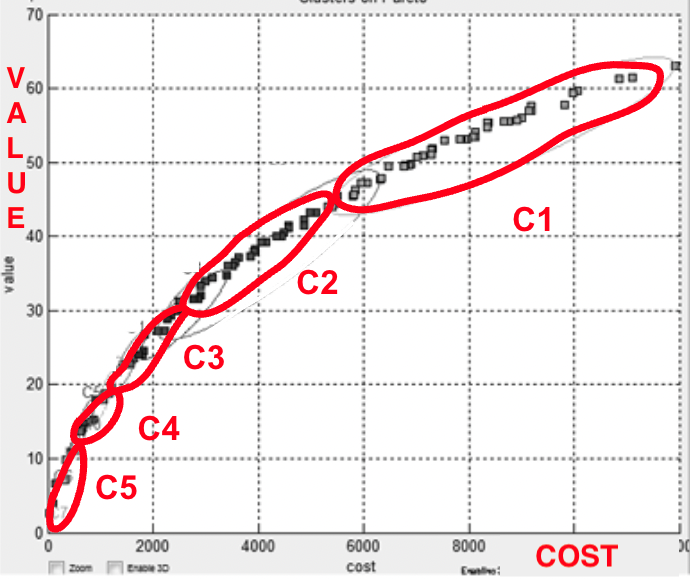
\includegraphics[width=2in]{img/frontier.png}
% \caption{ Veerappaization:  
% clusters of solutions seen in  (e.g.)  100s of   London ambulance designs,  grouped into 5 clusters. From~\cite{veerappa2011understanding}. }\label{Veerappa}\end{figure} 


% Returning now to the auditing problem that motivated this proposal,
%   divide-and-conqueror can dramatically reduce the effort required to compare trade-offs within a model.


%  \section{Data generation}

 
% Another   application for synthetic data  is privacy and the management of personnel and customer data.  Privacy regulations prevent sharing specific patient data. But companies and researchers can profit from sharing synthetic data that contains no one’s specific information, but only the aggregate insights.  For a longer list of applications of synthetic data, see Figure1

% provided that the data generator preserves     the desired properties of the original data, and does so with strong privacy mechanisms


% Not only can generated data mimic the original data, it can also selectively change some undesired properties. For example, synthesized data can be created that is sufficiently dissimilar from every individual, and can be tweaked in reduce biases in the data.   ``To build trust,” says Hazard in an IEEE Software article\footnote{To appear, Oct/Nov, 2023},  ``you can let anyone log in and look around. When they realize they can’t find themselves in the synthetic data, that is one more stakeholder willing to work with you''.

% Dr. Hazard reports a very large market for synthetic data. Recent changes to privacy legislation mean that soon, the whole AI industry will need to make much more use of fake data.  The European General Data Protection Regulation requires that personnel data be stored for the shortest time possible. Synthetic data offers a way around this clause. When the data is not personnel, but synthetic, then companies need not establish time limits to erase stored data.



% Synthetic data techniques can  create all the data needed to  satisfy the needs of  data hungry machine learning algorithms.  

% Synthetic data generation is also a method for making the data needed to stress test a system. 

% Synthetic data can change existing biases in data, thereby (e.g.) removing data discrimination.

% Synthetic data can be used to impute missing information in existing data.

% Synthetic data generated  can be used to enable data sharing, without incurring the wrath of legislative bodies. In this way, organizations can share insights, thereby assisting in scientific reasoning. 

% When most people work with the synthetic , not the real data, then this increases data security.

% Synthetic data can exploit current trends in data, thereby supporting forecasting.


% \section{Transparency and Interpretability}
% Transparency and interpretability are crucial aspects of AI systems, enabling users and stakeholders to understand how decisions are made. By employing software analytics techniques, we can gain insights into model behavior, feature importance, and decision processes. For instance, techniques like sensitivity analysis and rule extraction enable us to understand which inputs significantly influence the model's output, facilitating interpretability.
% Sensitivity analysis involves perturbing input features and observing the impact on the model's predictions. By identifying the most influential features, we can shed light on the decision-making process. Rule extraction techniques, such as decision tree induction or logical rule extraction, create interpretable models that mimic the behavior of complex AI models. These rule-based models provide insights into the decision logic and enable domain experts to validate and understand the AI system's behavior.

% \section{Robustness and Security}
% AI systems are vulnerable to adversarial attacks, wherein subtle modifications to input data can lead to incorrect predictions. Conventional software analytics techniques, such as static and dynamic analysis, can help identify vulnerabilities in AI models. By applying static analysis to examine model structure and dynamic analysis to detect runtime vulnerabilities, we can enhance the robustness and security of AI systems.
% Static analysis techniques analyze the code and structure of AI models to detect potential vulnerabilities. This includes identifying code patterns that may introduce vulnerabilities or analyzing the model's architecture for design flaws. Dynamic analysis, on the other hand, involves monitoring the model's behavior during runtime to detect anomalous or potentially malicious activities. By combining static and dynamic analysis, we can build AI models that are more resilient to attacks and ensure the integrity of their predictions.

% \section{Ethical Considerations and Fairness}
% Ensuring ethical considerations and fairness in AI systems is of paramount importance. AI systems must adhere to ethical principles and ensure fairness, avoiding biases based on race, gender, or other protected attributes. Conventional software analytics techniques, such as program slicing and data mining, can be utilized to detect and mitigate biases in training data and decision-making processes. By identifying discriminatory patterns, we can promote fairness and address societal concerns.
% Program slicing techniques isolate portions of the code that contribute to specific outputs or decisions. In the context of AI, program slicing can help identify discriminatory attributes or decision points that lead to biased outcomes. By addressing these biases, AI systems can provide fair and equitable results for all users. Data mining techniques can also be employed to analyze large datasets and identify biases in training data. By examining patterns and correlations, we can ensure that AI models are trained on diverse and representative datasets, minimizing biases in their predictions.

% \section{Handling Edge Cases}
% AI models often struggle with edge cases—uncommon or outlier scenarios that fall outside the training data distribution. By employing conventional software analytics techniques like anomaly detection and regression analysis, we can identify edge cases and develop more robust models. This enables AI systems to handle unforeseen scenarios and exhibit improved generalization capabilities.
% Anomaly detection techniques can help identify data instances that deviate significantly from the norm, thereby flagging potential edge cases. By incorporating these edge cases into the training process, AI models can learn to handle unusual scenarios more effectively. Regression analysis techniques can be used to model and understand the relationship between input features and predictions. This analysis helps identify regions in the input space where the model is likely to make errors or exhibit uncertain behavior. By addressing these areas, AI systems can make more reliable predictions in challenging scenarios.

% \section{Case Studies and Examples}
% To illustrate the potential of conventional software analytics in addressing open problems in AI, we present several case studies:
% \begin{itemize}
% \item
%  Using sensitivity analysis to identify discriminatory attributes in loan approval systems: By applying sensitivity analysis, we can understand which attributes disproportionately influence loan approval decisions. This enables financial institutions to ensure fairness and reduce biases, fostering equal opportunities for all applicants.
% \item  Applying static analysis to detect vulnerabilities in autonomous vehicle perception models: Static analysis techniques can uncover potential vulnerabilities in the perception models used by autonomous vehicles. By identifying security flaws early in the development process, we can enhance the robustness and safety of these systems, protecting against potential attacks and ensuring passenger safety.
% \item  Leveraging program slicing to identify potential security vulnerabilities in natural language processing models: Program slicing can help isolate code segments that contribute to specific decisions in natural language processing models. By analyzing these code segments, we can identify potential security vulnerabilities and strengthen the confidentiality and integrity of user data.
% % \end{itemize}
 
% This paper advocates for the integration of conventional software analytics techniques to address open problems in AI. By leveraging the vast array of tools and methodologies developed in the software engineering domain, we can enhance the transparency, interpretability, robustness, fairness, and handling of edge cases in AI systems. The proposed approach offers promising avenues for further research and development, paving the way for the responsible and ethical deployment of AI technologies in various domains. By combining the power of AI and software analytics, we can overcome the existing challenges, unlocking the full potential of AI for the benefit of society.

\balance
 \bibliographystyle{ACM-Reference-Format}
\bibliography{acmart}







\end{document}
